\chapter{Проектирование и разработка программных средств решения задачи сегментации и классификации крюков}

\section{Проектирование и разработка программных средств генерации редактируемой цифровой копии страницы с крюками и знамёнами}

\subsection{Требования к реализации}

Проектирование модели ведется в рамках работы над порталом, поэтому основные требования к ней 
исходят из задач и потребностей самого портала. Основной целью является создание системы, 
способной эффективно работать с текстами рукописного наследия, обеспечивая высокую скорость 
сегментации и классификации крюков и знамён.

Исходя из этого, основными требованиями к системе являются\cite{MLeffinguel}:
\begin{itemize}
  \item Сегментация и классификация крюков на изображении: Система должна анализировать 
    входное изображение, выделять области, содержащие крюки, и определять их контуры и 
    границы. Затем система должна классифицировать каждый выделенный крюк по 
    классам, используя метод шаблонного сопоставления. 
  \item Хранение данных: Система должна сохранять результаты сегментации и классификации 
    в виде количества крюков на странице. Для каждого крюка должны сохраняться 
    его координаты на изображении и его класс.
  \item Простая расширяемость: При дальнейшем дообучении модели на более ранних текстах 
    (например, XVIII века) необходимо, чтобы система распознавания могла быть легко 
    адаптирована для работы с новыми данными. Это обеспечит возможность расширения 
    функционала модели без значительных модификаций её архитектуры, гарантируя её 
    актуальность на протяжении долгого времени.
  \item Эффективность работы и скорость выполнения: Основной задачей модели является определение необходимости 
    запуска нейросети. Время её работы должно быть сведено к минимуму, чтобы 
    обеспечить высокую производительность портала. Это потребует оптимизации 
    алгоритмов и внедрения эффективных методов обработки данных, чтобы 
    пользователи могли получить результаты в кратчайшие сроки.
\end{itemize}


Архитектура системы распознавания портала представлена в виде:
\begin{figure}[H]
  \begin{center}
    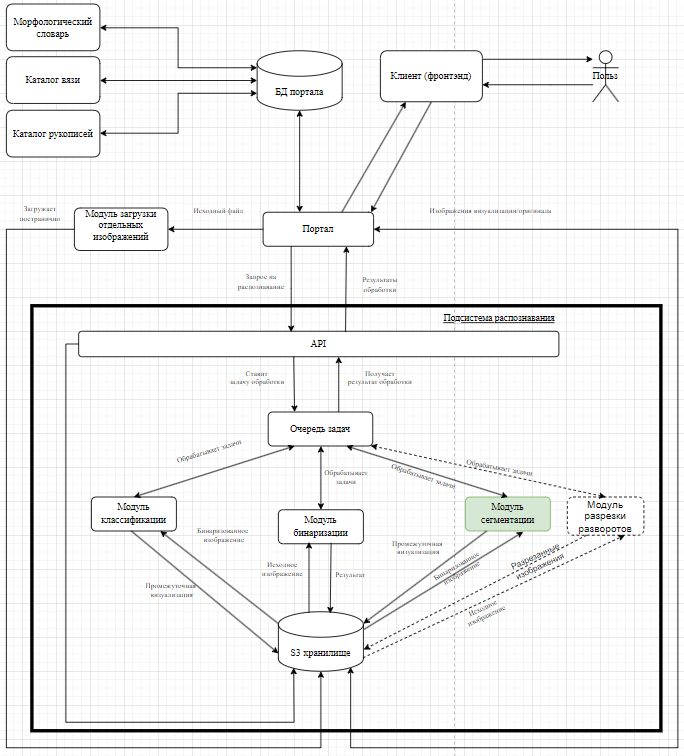
\includegraphics[width=.8\columnwidth]{./img/portal_Arh.png}%
  \end{center}
  \caption{Архитектура системы распознавания.}%
  \label{pic:portalArh}%
\end{figure}

\subsection{Модификация модуля сегментации}

Архитектурно, модуль сегментации имеет вид:

\begin{figure}[H]
  \begin{center}
    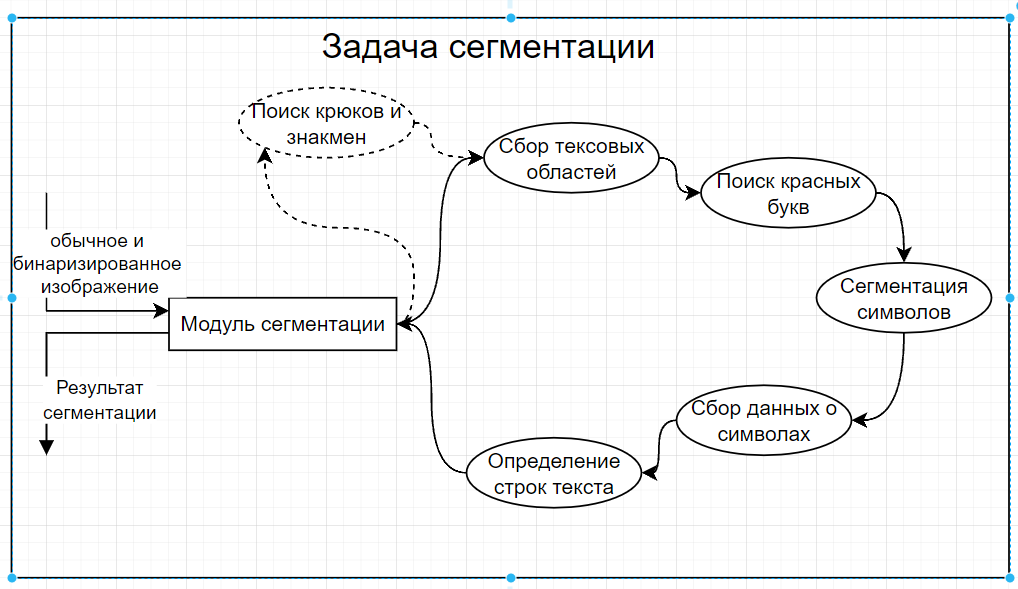
\includegraphics[width=.7\columnwidth]{./img/segment_module.png}%
  \end{center}
  \caption{Архитектура модуля сегментации.}%
  \label{pic:segment_module}%
\end{figure}

Модулю ставится на вход задача сегментации изображения, на вход присылается обычное и 
бинаризированное изображение, после завершения обработки, модуль возвращает результат.

Для поиска крюков и знамен не требуется результат работы компонент модуля, поэтому не следует
встраивать ее в общий пайплайн сегментации, что бы не путать разработчиков. Хорошим вариантом ее 
расположения будет или до начала пайплайна или по его завершению. На рис. \ref{pic:segment_module}
новая компонента модуля выделена пунктиром.

\begin{figure}[H]
  \begin{center}
    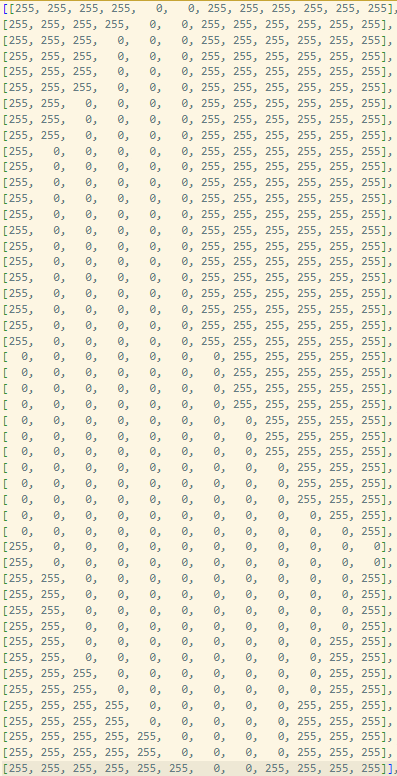
\includegraphics[width=.4\columnwidth]{./img/binmask.png}%
  \end{center}
  \caption{Пример бинарной маски крюка.}%
  \label{pic:segment_module}%
\end{figure}

Выбор бинарных масок крюков в качестве модели представления является хорошим решением для работы 
с древнеславянскими рукописями. Такие маски создаются на основе выборки изображений крюков и 
обеспечивают множество преимуществ при их последующем использовании.

\begin{itemize}
  \item Высокая точность определения форм.
  \item Универсальность, бинарная маска одного и того же крюки при грамотном указании точности соответствия подходит
    для поиска подавляющего кол-ва соответствующих крюков.
  \item Быстрота исполнения из-за их легковесности.
\end{itemize}


\section{Интеграция программных средств сегментации в портал Корпуса рукописного наследия Древней Руси}

Для реализации алгоритма шаблонного сопоставления была выбрана библиотека OpenCV с методом cv2.matchTemplate.
Этот метод очень хорошо оптимизирован, за счет многопоточной обработки, и реализации на C++.

Результаты поиска крюков с использованием бинарных масок следует хранить в виде количества найденных крюков и 
их точного расположения. Для представления расположения крюков был выбран формат JSON. Этот формат позволяет 
структурированно и наглядно описывать характеристики найденных объектов, такие как класс символа и координаты 
его местоположения. 

\begin{figure}[H]
  \begin{center}
    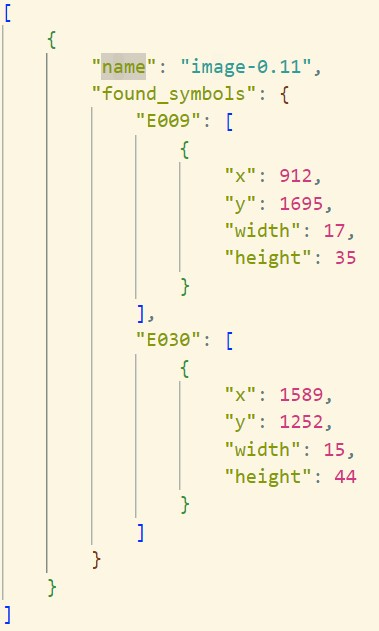
\includegraphics[width=.5\columnwidth]{./img/jsonModel.jpg}%
  \end{center}
  \caption{Пример Json файла для обработаного изображения.}%
  \label{pic:jsonModel}%
\end{figure}

Дополним задачу tasks.segment, являющуюся основной в модуле сегментации. Перед сегментации изображений
запустим поиск крюков с помощью cv2.matchTemplate, на основе наших бинарных масок, указав точность
соответствия в 85\%.

Результат работы сегментации крюков запишем в результат работы модуля сегментатора.

Полученные в результате вызова API данные сегментации стоит записать в базу данных портала, для этого проведем
миграцию базы данных Images, добавив колонку hooks, отвечающую за кол-во найденных крюков.

БД портала основана на СУБД PostgreSql, миграции осуществляются посредством alembic, что позволяет автоматизировать
этот процесс.

\section{Выводы}

В результате проектирования модели и архитектуры для решения задачи сегментации и классификации 
крюков, полученная модель является легковесной, быстрой и легко расширяемой, посредством увеличения выборки.

% \begin{figure}[H]
%   \begin{center}
%     \includegraphics[width=.9\columnwidth]{./img/binmasks.png}%
%   \end{center}
%   \caption{Пример бинаризированыных масок крюка E012.}%
%   \label{pic:binmasks}%
% \end{figure}

%%% Local Variables:
%%% TeX-engine: xetex
%%% eval: (setq-local TeX-master (concat "../" (seq-find (-cut string-match ".*-3-pz\.tex$" <>) (directory-files ".."))))
%%% End:
